\documentclass{standalone}
\usepackage{tikz}
\usepackage{xcolor}
\usepackage{amsmath}

\usetikzlibrary{shapes.geometric, arrows.meta, positioning}

\tikzstyle{layer} = [rectangle, draw, minimum height=1cm, minimum width=2cm, align=center]
\tikzstyle{arrow} = [thick, -{Stealth}]

\begin{document}

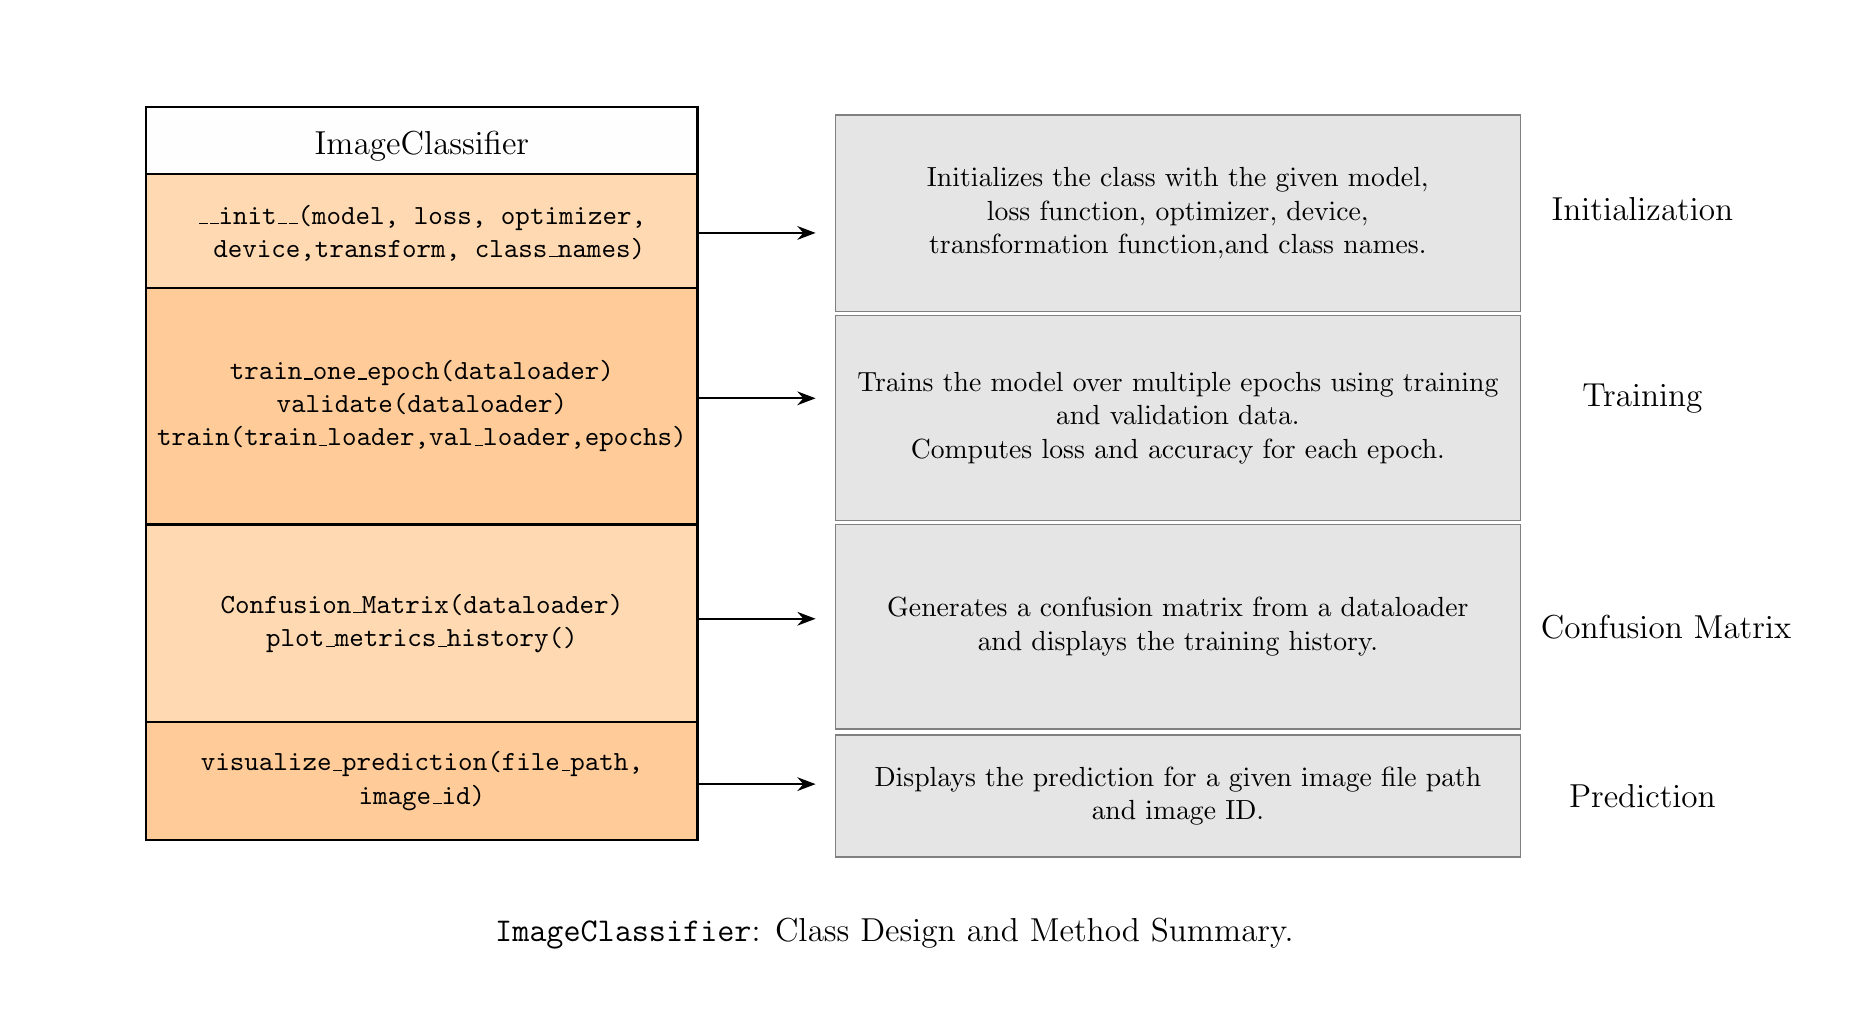
\begin{tikzpicture}[node distance=1.5cm and 1.5cm]
\draw[rectangle,draw=white](0,0)--(23,12);
\node[layer, fill=lightgray!1, draw=black, minimum width=7cm,  minimum height=8cm, line width=.8pt,  align=center] (input) at (5,7) {Input};
\node[](input) at (5,10.5) {\large ImageClassifier}; 
\draw[line width=.8pt, draw=black] (1.74,10) -- (8.24,10);
\node[layer, fill=orange!30, draw=black, minimum width=7cm,  minimum height=1.5cm, line width=.8pt,  align=center] (input) at (5,9.4) {\texttt{\_\_init\_\_(model, loss, optimizer,}\\\texttt{ device,transform, class\_names)}};

\node[layer, fill=orange!40, draw=black, minimum width=7cm,  minimum height=3cm, line width=.8pt,  align=center] (input) at (5,7.2) 
                {\texttt{train\_one\_epoch(dataloader)}\\
                \texttt{validate(dataloader)}\\
                \texttt{train(train\_loader,val\_loader,epochs)}};

\node[layer, fill=orange!30, draw=black, minimum width=7cm,  minimum height=2.5cm, line width=.8pt,  align=center] (input) at (5,4.44)
                {\texttt{Confusion\_Matrix(dataloader)}\\
                \texttt{plot\_metrics\_history()}};
\node[layer, fill=orange!40, draw=black, minimum width=7cm,  minimum height=1.5cm, line width=.8pt,  align=center] (input) at (5,2.44)
                {\texttt{visualize\_prediction(file\_path, }\\
                  \texttt{image\_id)}};
\draw[arrow] (8.5,9.4)--(10,9.4);
\node[layer, fill=lightgray!40, draw=black!50, minimum width=8.7cm,  minimum height=2.5cm, line width=.5pt,  align=center] (input) at (14.6,9.65) {Initializes the class with the given model, \\loss function, optimizer, device,\\ transformation function,and class names.};
\draw[arrow] (8.5,7.3)--(10,7.3);
\node[layer, fill=lightgray!40, draw=black!50, minimum width=8.7cm,  minimum height=2.6cm, line width=.5pt,  align=center] (input) at (14.6,7.05) {Trains the model over multiple epochs using training \\and validation data. \\Computes loss and accuracy for each epoch.};                 
\draw[arrow] (8.5,4.5)--(10,4.5);
\node[layer, fill=lightgray!40, draw=black!50, minimum width=8.7cm,  minimum height=2.6cm, line width=.5pt,  align=center] (input) at (14.6,4.4) {Generates a confusion matrix from a dataloader\\ and displays the training history.};
\draw[arrow] (8.5,2.4)--(10,2.4);
\node[layer, fill=lightgray!40, draw=black!50, minimum width=8.7cm,  minimum height=1.55cm, line width=.5pt,  align=center] (input) at (14.6,2.25) {Displays the prediction for a given image file path \\and image ID. };
\node[layer,draw=white, minimum width=3cm,  minimum height=1.5cm, align=center] (input) at (20.5,9.7) {\large Initialization};
\node[layer,draw=white, minimum width=3cm,  minimum height=1.5cm, align=center] (input) at (20.5,7.3) {\large Training};
\node[layer,draw=white, minimum width=3cm,  minimum height=1.5cm, align=center] (input) at (20.8,4.4) {\large Confusion Matrix};
\node[layer,draw=white, minimum width=3cm,  minimum height=1.5cm, align=center] (input) at (20.5,2.25) {\large Prediction};
\node[layer,draw=white, minimum width=3cm,  minimum height=1.5cm, align=center] (input) at (11,0.5) {\large \texttt{ImageClassifier}: Class Design and Method Summary.};
\end{tikzpicture}

\end{document}
